%Centralizar verticalmente.
\newenvironment{midpage}{\vspace*{\fill}}{\vspace*{\fill}}
%Centralizar horizontalmente.
\newenvironment{midline}{\hspace*{\fill}}{\hspace*{\fill}}
\documentclass[12pts]{article}
\usepackage[utf8]{inputenc}
%Pacote para colocar cor no código.
\usepackage{color}
\definecolor{light-gray}{gray}{0.95}
%Pacote para inserir código.
\usepackage{listings}
\lstset{
    numbers=left,
    tabsize=2,
    backgroundcolor=\color{light-gray},
}
\title{
	Prática de Eletrônica Digital 1 - (119466)
	\singlespacing
		Turma E (Unb - Gama)
	\singlespacing
	\begin{midpage}
	\begin {large}
		Pré-Relatório Experimento 5
		\singlespace
		Circuitos Multiplexadores e Demultiplexadores
	\end {large}
	\end{midpage}
}
\date{Setembro 27, 2016}
\usepackage{indentfirst}
\usepackage{setspace}
\usepackage{verbatim}
\usepackage[pdftex]{hyperref}
\usepackage{graphicx}
\begin{document}
\maketitle	
%\vspace{100 mm}
\begin{center}

\begin{tabular}{|c|l|r|}
\hline
Nome & Matrícula & Assinatura\\
\hline
Arthur Temporim & 140016759 & \\
\hline	
Eduardo Nunes & 140056149 & \\
\hline	
\end{tabular}

\end{center}

\pagebreak

\section{Projetos e Simulações}

	Na seção a seguir contém as atividades pedidas para a elaboração do pré-relatório.
	
\subsection{Projeto1 - Decodificador com Mux}
\subsubsection{Diagrama Esquemático}

\textbf{Diagrama Projeto1 - Decodificador:}

\begin{figure}[!htb]
  \centering
  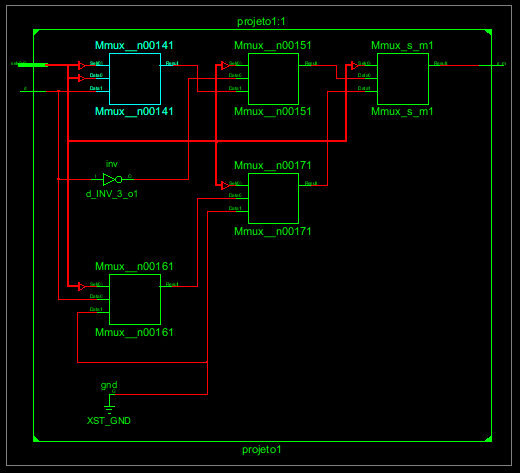
\includegraphics[scale=0.7	]{imagens/esquematico_projeto1}
  \caption{Diagrama 1 - Ise Design Suit 14.7}
  \label{figRotulo}
\end{figure}

\newpage
\subsubsection{Código VHDL}

\lstinputlisting[language=vhdl]{projetos/projeto1/projeto1.vhd}

\clearpage

\subsection{Projeto2 - Multiplexar display}

	Este projeto consiste na utilização de 2 displays de 7 segmentos utilizando apenas 1 multiplexador e 1 decodificador BCD, também foram permitidos o gerador de função para gerar o \textit{clock} e o seletor de dispositivo.
	
	Toda a implementação do circuito abaixo foi feita diretamente em VHDL, os esquemáticos gerados foram feitos a partir da ferramenta. Porém a compreensão do circuito foi fornecida através do diagragam de blocos (figura 5.6) do roteiro experimental.
	
	Devido à esta abstração, não foi necessário a construção do circuito em forma de esquemático.

\subsubsection{Diagrama Esquemático}

\textbf{Diagrama Projeto2 - Multiplexador:}

\begin{figure}[!htb]
  \centering
  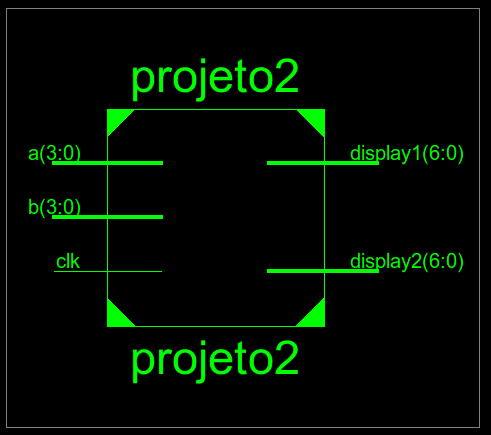
\includegraphics[scale=0.7	]{imagens/esquematico_projeto2macro}
  \caption{Esquematico macro do projeto 2 - Ise Design Suit 14.7}
  \label{figRotulo}
\end{figure}

\clearpage

\begin{figure}[!htb]
  \centering
  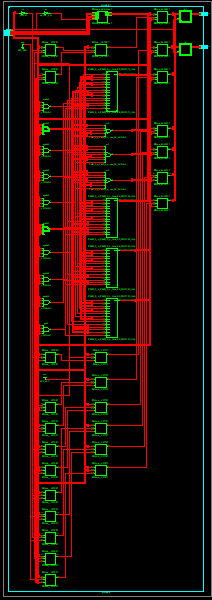
\includegraphics[scale=0.7	]{imagens/esquematico_projeto2}
  \caption{Esquematico geral do projeto 2 - Ise Design Suit 14.7}
  \label{figRotulo}
\end{figure}


\clearpage
\subsubsection{Código VHDL}

\lstinputlisting[language=vhdl]{projetos/projeto2/projeto2.vhd}

\clearpage
\subsubsection{Testes do projeto}

\begin{figure}[!htb]
  \centering
  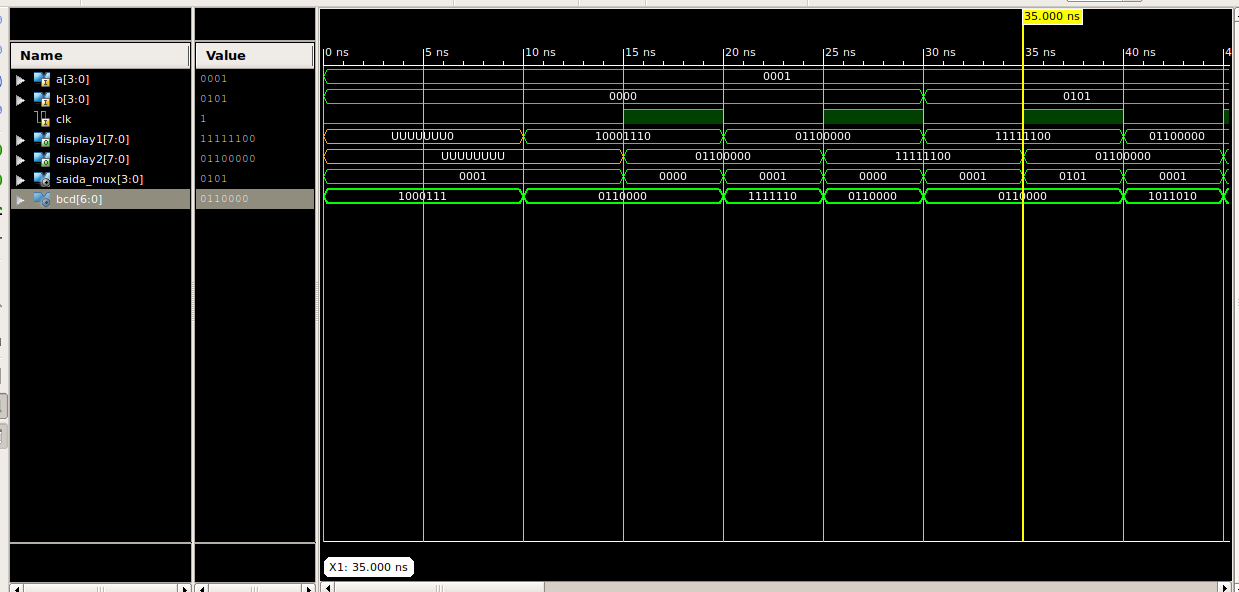
\includegraphics[scale=0.35	]{imagens/onda_projeto2}
  \caption{Forma de onda do projeto 2 - Ise Design Suit 14.7}
  \label{figRotulo}
\end{figure}

\end{document}
